\newenvironment{definition}[1][Definition]{\begin{trivlist}
\item[\hskip \labelsep {\bfseries #1}]}{\end{trivlist}}

\chapter{Overview}
\label{c:overview}
An overview of the proposed 3D head motion tracking system is illustrated in this chapter. In Section \ref{s:problem}, we give a clear definition for our head motion tracking task. After that, the introduction of the hardware is illustrated in Section \ref{s:hardware}. We will discuss the pros and cons of the hardware, and specify the output format of this device so that the input data of the proposed system can be clear. Section \ref{s:architecture} shows the software system architecture of this system. A high level introduction of the work flow is specified here before going into the implementation details of this work which is specified in Chapter \ref{c:method}. We show our results in Chapter \ref{c:result}. Conclusion and future work are discussed in Chapter \ref{c:conclusion}.

\section{Problem Formulation}
\label{s:problem}
The goal of 3d head motion tracking is to recover the transformation of a person's head in 3D space. The transformation includes rotations with respect to and translations along the three axes. For clear, we give it a definition as the following:
\begin{definition}
The 3D head motion tracking task is the real-time recovery of the six degree of freedom head pose vector of the target head in 3D space given a stream of live performed depth maps.
\end{definition}
In the definition, the head pose vector is a 6$\times$1 vector $v = (r_{x},r_{y},r_{z},t_{x},t_{y},t_{z})^{T}$, which is consisted of six parameters, three of them are the rotation parameters $(r_{x},r_{y},r_{z})^{T}$ and rest of them are the translation parameters $(t_{x},t_{y},t_{z})^{T}$ of the target head in a 3D space.
\begin{figure}
\centering
\includegraphics[width=0.5\linewidth]{./figure/yawpitchroll.pdf}
\caption{Illustration of the three degrees of freedom rotation. Pitch, yaw, and roll are the rotating angle of three mutual orthogonal directions.}
\label{f:rollpitchyaw}
\end{figure}

Figure \ref{f:rollpitchyaw} illustrates the rotation parameters where $r_{x}$ indicates the angle that the head rotates around the $x$-axis, $r_{y}$ indicates the angle that the head rotates around the $y$-axis and $r_{z}$ indicates the angle that the head rotates around the $z$-axis. Borrowing aviation terminology, these rotations are commonly referred to as pitch, yaw, and roll. Pitch angle equals to $r_{x}$; Yaw angle equals to $r_{y}$; Roll angle equals to $r_{z}$. As a more life style description, pitch indicates the motion that the user nods his head, yaw indicates the motion that the user shakes his head left or right, roll indicates the motion that the user tilts his head.

 
\section{Hardware}
\label{s:hardware}
In this thesis, we adopt a depth sensor as our system's input device. Noted that a depth camera is also known as a range camera, and depth data is also known as range data. Instead of those high level depth sensors such as \emph{SwissRanger SR4000}  by \emph{Messa Imaging} which was priced at \$9000 USD or \emph{CamCube} by \emph{PMD Technologies} which was priced at \$12000, we choose the consumer affordable depth cameras such as \emph{XBox Kinect} by \emph{Microsoft} or \emph{Xtion Pro} by \emph{ASUS}, both of them were priced at about \$150 USD.
Xbox Kinect is a motion sensing input device designed for XBox 360 video game console. It was promoted by Microsoft on November, 2010. Kinect is able to capture a color image and its corresponding depth map simultaneously at 30 frames per second, both with a display resolution of 640$\times$480. A similar device named Xtion Pro Live is also released in the same time by ASUS. Figure \ref{f:kinect} shows the devices and the data captured by them, the upper row is Kinect while the lower row is Xtion Pro Live.
\begin{figure}
\centering
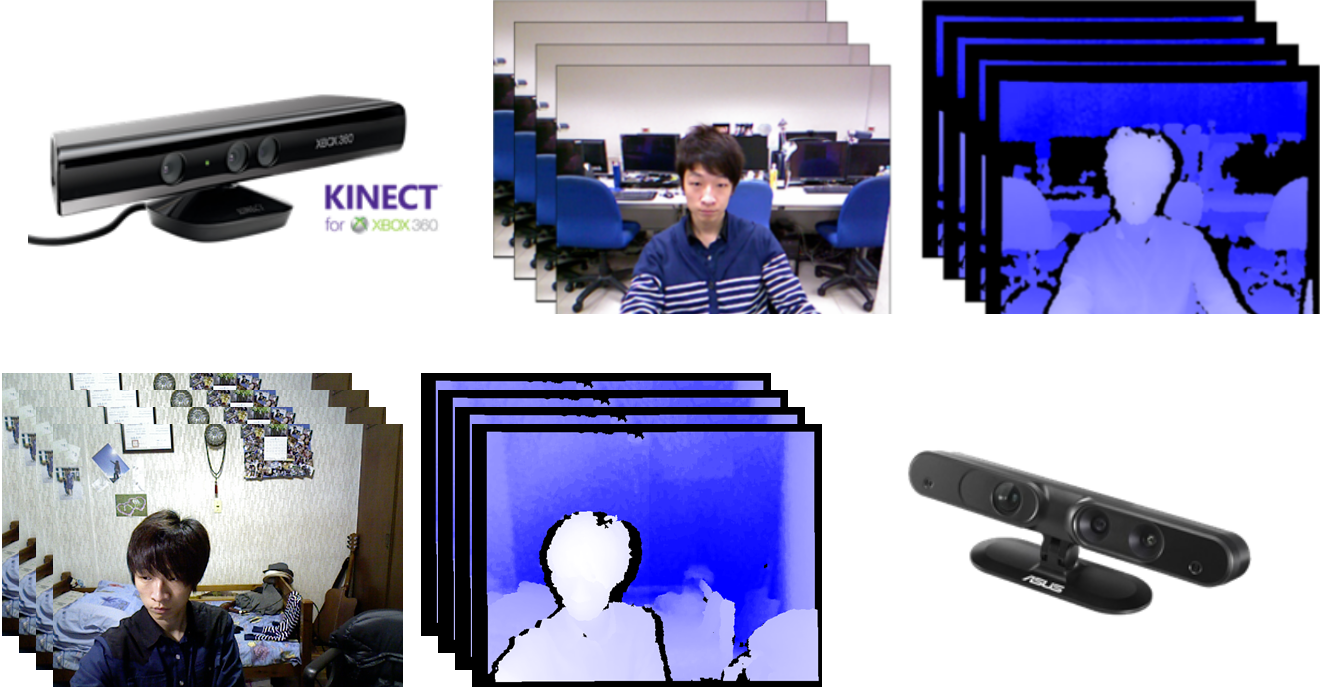
\includegraphics[width=1.0\linewidth]{./figure/kinect.png}
\caption{The color image and the corresponding depth map captured by Kinect and Xtion Pro Live, both with resolution of 640$\times$480 at 30 fps.}
\label{f:kinect}
\end{figure}

The sensors with which Kinect equipped including an infrared ray emitter, a visible light camera, an infrared ray receiver, a microphone array and a pedestal motor. While many advanced depth cameras use \emph{``time-of-flight(ToF)''} technique to calculate the distance from the camera to an object by measuring the time it takes for a beam of light to travel to and reflect back from the object's surface, Kinect uses a totally different technique called \emph{``light coding''}. The emitter emits infrared ray which pass through a filter and is scattered into a fixed pattern of speckles. These speckles are then projected onto the scene, see Figure \ref{f:irspeckles}.
\begin{figure}
\centering
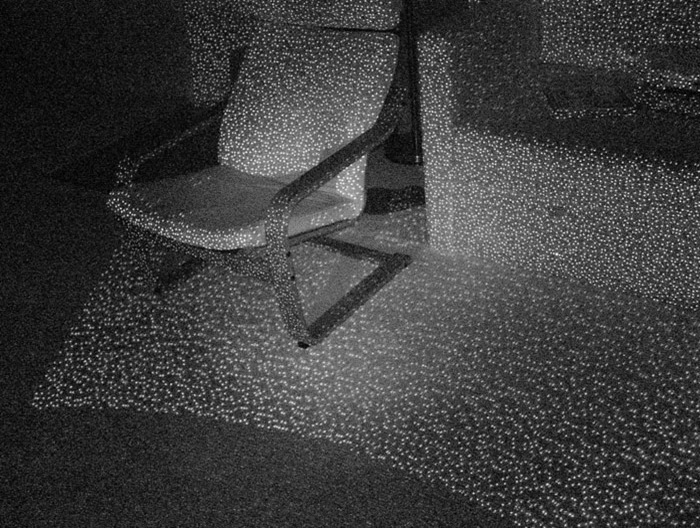
\includegraphics[width=0.5\linewidth]{./figure/irspeckles.jpg}
\caption{The projected infrared ray speckles, captured by SONY F717.}
\label{f:irspeckles}
\end{figure}
The reflected pattern, which reveals the distribution of the speckles thus contains the geometrical information of the scene, is then captured by the IR receiver. After decoding the reflected IR pattern, the distance between the camera and the surfaces of object in the scene can be determined, and the corresponding depth map is available.

In brief, Kinect is a non-intrusive, commercially available and consumer affordable device of which the deployment is as easy as an ordinary camera. Furthermore, the user is not required to wear any sensors or markers on his body. The quality of the acquired depth map is not affected by illumination variations.

However, the advantages of this acquisition device come at the cost of high level noises in the acquired data. There is a flicker problem within the acquired depth maps. It is caused by the combination of depth value fluctuation and depth value loss. Our experiments show that the range of fluctuation is about 0.5\% of the distance from the obserced object to the camera in average. That is to say, the error range of every pixel on the depth map is within 0.5cm when the user stands 100cm away from Kinect. Besides, when the IR rays are blocked from being received by Kinect, or there's actually no IR rays reflected from the object surfaces, the depth value of the corresponding pixel on the depth map would be lost. These are caused by specular reflections, transparent materials the horizontal disparity between the IR emitter and the IR receiver, and occlusions. As a consequence, we should handle these issues carefully.

\section{System Architecture}

\begin{figure}
\centering
\includegraphics[width=1.0\linewidth]{./figure/visualflowchart.pdf}
\caption{Visualized work flow of our system. The depth sensor captures the user's actions in real-time, a stream of depth maps is created and is the input of our system. Two methods, least square error method and iterative optimization method, are then applied to do the head motion tracking. The estimated motion vectors are then used to animate virtual avatars at last.}
\label{f:visualized flow chart}
\end{figure}

A high level work flow visualization of our system is illustrated in Figure \ref{f:visualized flow chart}. The depth sensor captures the user's head motion performance in real-time. A stream of depth maps is then created and passed into our system as input data. The third block is the main part of the proposed approach of head pose estimation. Two methods are proposed independently, least square error method and iterative optimization method. Both of them are able to complete the work along. This part which will be discussed in detail in Chapter \ref{c:method}. The fourth block shows that we can retarget the estimated head poses to virtual characters.


\begin{figure}
\centering
\includegraphics[width=1.0\linewidth]{./figure/m1FlowChart.pdf}
\caption{Detailed flow chart of the first proposed motion tracking algorithm which applies least square error method to accomplish the goal.}
\label{f:m1 flow chart}
\end{figure}

Figure \ref{f:m1 flow chart} shows a more detailed flow chart about the first proposed method. This method starts with depth map acquisition for each frame followed by a nose detecting/tracking process. Then we separately accomplish the roll, yaw, pitch angels estimation by two stages: One is to solve a least square error plane approximating to the frontal face for the yaw and pitch angels; The other one is to solve a least square error ellipse approximating to the head's contour for the roll angel. As a result, the nose position shows the former three degree of freedom of the motion vector while the least square methods tells the rest three. The 6-DoF motion vector is then solved. However, the resulting animation driven by these frame by frame motion vectors still has a serious trembling issue. This is mainly because of the low quality of the input depth map. We apply a dynamic weighted averaging filter references from \cite{Weise:11:RPBFA} to tackle this issue. The output of the filter is the final result of this method. This approach performs well in response time which is 30 fps. This makes the system able to give users good experiences. However, when it comes to the precision, the exact number of the rotation angles comparing with the ground truth, it will not show good statistical results.

\begin{figure}
\centering
\includegraphics[width=1.0\linewidth]{./figure/m2FlowChart.pdf}
\caption{Detailed flow chart of the second proposed motion tracking algorithm which applies iterative optimization method to accomplish the goal.}
\label{f:m2 flow chart}
\end{figure}
\label{s:architecture}

In order to improve the precision of the system, we decide to replace the least square error method by optimization method. In order to retain the real-time feature, we design the optimization to be aimed at a sparse-to-dense point cloud matching, which means to find the best match between an on-line sparsely sampled point cloud and an user specific densely sampled model point cloud. We will show that the model point cloud is still on-line created in Chapter \ref{c:method} so that this will not cause a time consuming off-line preparation as the approach in \cite{Weise:11:RPBFA}. Figure \ref{f:m2 flow chart} shows a detailed flow chart about the proposed optimization method. The architecture of this method is similar to the previous one. Blocks which are circled by dotted lines are the different parts between two methods. At the very beginning of the system, the user can choose to load his head model point cloud which has been off-line created, or the user can choose to directly start the on-line motion tracking process with his head facing the depth camera. In the former case, the system loads a point cloud and create a KD-tree index. In the latter case, the system takes the first captured frame to create an user specific densely sampled model point cloud and its KD-Tree index. Both of the cases take about 30 ms which the user can hardly be aware of. After the nose position is detected, a sample point cloud is sparsely sampled from the nose's nearby area. We define an objective function which measures the distance between the sample point cloud and the model point cloud, and adopt gradient decent algorithm to iteratively optimize this function. As the iterative process converges, we obtain the 6-DoF motion vector, too. 